\label{sect:LayerDesc}
This section describes the \textit{responsible softmax layer} as a method to use \DR in approximating class weights \( \hat{\bm \pi} \) and class density functions \( f_i(x) \). The responsible softmax layer uses a combination of dynamic responsibility and backpropagation to determine class weights \( \hat{\bm \pi} \) for weighting a typical softmax layer.  While weighted softmax layers are not new, the typical approach is to apply the same weight for every class.  This weight is either set as a hyper parameter, or is occasionally determined through backpropagation.  On the occasion that multiple class weights are used, they are usually set once to proportions determined \textit{a priori} by class labels \( T \) and are not learned parameters.  Chapter \ref{ch:experiments} discusses when each approach might be reasonable.

To discuss responsible softmax (RS), understanding of weighted softmax is required.  Recall from section \ref{softmax} equation \ref{eqn:softmaxDef} that softmax is the multivariable extension of the logistic function. A weighted softmax adds multiplication weights to each exponential function in the usual softmax \textit{i.e.}
\begin{equation}\label{eqn:weightSoftmax}
\gs_i(\bm x,\bm\gb) = \dfrac{e^{x_i\gb_i}}{\sum_j e^{x_j\gb_j}}.
\end{equation}
Equation \ref{eqn:weightSoftmax} for weighted softmax is very similar to equations \ref{softResp} and \ref{emResp} from chapter \ref{ch:background}. One paper that uses a weighted softmax approach is that of Liu et. al. \cite{liu2016large}. This paper defines \( L \)-softmax, which gives a different weight to each class. 

Another brief discussion for weighting the softmax loss is implied in Bishop \cite[sect. 6.5]{Bishop1995}.  Bishop frames the discussion there in terms of compensating for different priors.  If \( \tilde{\!\bm\pi} \) is defined by \( \tilde{\!\pi}_i = \#\{t_i^{n}\in T|t_i^{n}=1\}/N \), \textit{i.e.} the proportion of training targets with class \( i \), then compensating for that prior is what this dissertation calls \textit{empirically weighted softmax}.  This name is chosen as the weights are determined empirically from the training targets \( T \).

Responsible Softmax uses the predictor \( Y \) as described in equation \ref{Ydef}.  As seen in equation \ref{eqn:YdefLogcoords}, this is similar to adding a bias element in the fully connected layer before the softmax layer. Responsible softmax differentiates itself from using a bias in that the wights \( \mu_i = \log\pi_i \) are not determined by backpropagation, but through dynamic responsibility.  This also distinguishes RS from other weighted softmax methods in that the multiplicative weight is not on the output of a fully connected layer, but on the exponentiation of that output.

\begin{figure}[h]
	\centering
	\usetikzlibrary{decorations.pathreplacing}
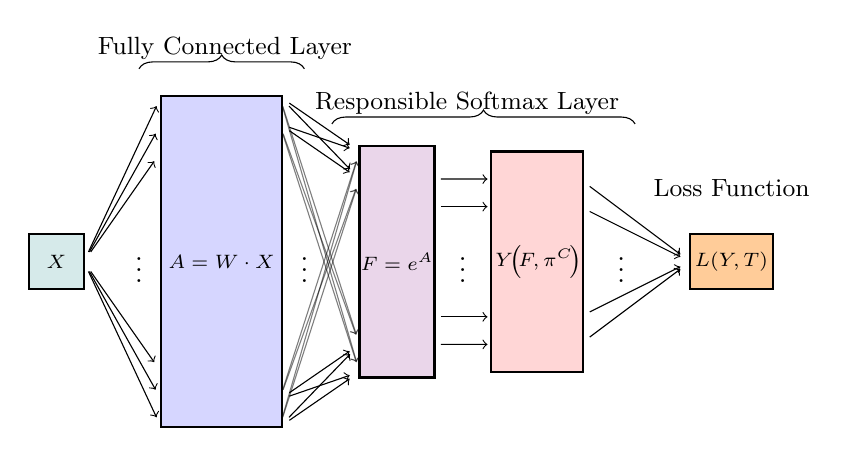
\begin{tikzpicture}[scale = .7]
% Layer boxes and labels
\draw  [fill = teal!20, fill opacity = .8, thick ](-7.5,0) rectangle (-6.5,-1);
\node at (-7,-0.5) {\scriptsize$\bm X$};
\draw  [fill = blue!20, fill opacity = .8, thick ](-5.1,2.5) rectangle (-2.9,-3.5);
\node at (-4,-0.5) {\scriptsize\(\bm A =\bm W\cdot \bm X\)};
\draw  [fill = violet!20, fill opacity = .8, thick ](-1.5,1.6) rectangle (-0.14,-2.6);
\node at (-.815,-0.5) {\scriptsize$\bm F = e^{\bm A}$};
\draw  [fill = red!20, fill opacity = .8, thick ](.88,1.5) rectangle (2.55,-2.5);
\node at (1.75,-0.5) {\scriptsize$\bm Y\!\!\left(\!\bm F,\bm\pi^C\!\right)$};
\draw  [fill = orange!50, fill opacity = .8, thick ](4.5,0) rectangle (6,-1);
\node at (5.25,-0.5) {\scriptsize$L(\bm Y,\bm T)$\normalsize};
% Connections between first and second layer
\node (v1) at (-6.5,-0.5) {};
\node (v2) at (-5.1,2.5) {};
\node (v3) at (-5.1,2) {};
\node (v4) at (-5.1,1.5) {};
\node at (-5.5,-0.5) {{$\vdots$}};
\node (v6) at (-5.1,-3) {};
\node (v7) at (-5.1,-3.5) {};
\node (v5) at (-5.1,-2.5) {};
\draw [->] (v1) edge (v2);
\draw [->] (v1) edge (v3);
\draw [->] (v1) edge (v4);
\draw [->] (v1) edge (v5);
\draw [->] (v1) edge (v6);
\draw [->] (v1) edge (v7);
% Connections between second & 3rd layer
\node (v8) at (-2.95,2.5) {};
\node (v11) at (-2.95,2) {};
\node (v15) at (-2.95,-3) {};
\node (v12) at (-2.95,-3.5) {};
\node (v9) at (-1.5,1.5) {};
\node (v10) at (-1.5,1) {};
\node (v14) at (-1.5,-2) {};
\node (v13) at (-1.5,-2.5) {};
\draw [->] (v8) edge (v9);
\draw [->] (v8) edge (v10);
\draw [->] (v11) edge (v9);
\draw [->] (v11) edge (v10);
\draw [->] (v12) edge (v13);
\draw [->] (v12) edge (v14);
\draw [->] (v15) edge (v13);
\draw [->] (v15) edge (v14);
\draw [->,opacity = .5] (v8) edge (v14);
\draw [->,opacity = .5] (v8) edge (v13);
\draw [->,opacity = .5] (v11) edge (v14);
\draw [->,opacity = .5] (v11) edge (v13);
\draw [->,opacity = .5] (v15) edge (v9);
\draw [->,opacity = .5] (v15) edge (v10);
\draw [->,opacity = .5] (v12) edge (v9);
\draw [->,opacity = .5] (v12) edge (v10);
\node at (-2.5,-0.5) {{$\vdots$}};
% Connections between 3rd and 4th layer
\node (v16) at (-0.2,1) {};
\node (v18) at (-0.2,0.5) {};
\node (v20) at (-0.2,-1.5) {};
\node (v22) at (-0.2,-2) {};
\node (v23) at (1,-2) {};
\node (v21) at (1,-1.5) {};
\node (v19) at (1,0.5) {};
\node (v17) at (1,1) {};
\draw [->] (v16) edge (v17);
\draw [->] (v18) edge (v19);
\draw [->] (v20) edge (v21);
\draw [->] (v22) edge (v23);
\node at (0.375,-0.5) {{$\vdots$}};
% Connections between 4th and 5th layer
\node (v25) at (4.5,-0.5) {};
\node (v24) at (2.5,1) {};
\node (v26) at (2.5,0.5) {};
\node (v27) at (2.5,-1.5) {};
\node (v28) at (2.5,-2) {};
\draw [->] (v24) edge (v25);
\draw [->] (v26) edge (v25);
\draw [->] (v27) edge (v25);
\draw [->] (v28) edge (v25);
\node at (3.25,-0.5) {{$\vdots$}};
% Layer labels
\draw [decorate,  decoration={brace,  amplitude=5pt}] (-5.5,3)--(-2.5,3) node[above, xshift =-28.7]{\small Fully Connected Layer};
\draw [decorate,  decoration={brace,  amplitude=5pt}] (-2,2)--(3.5,2) node[above, xshift =-60.7]{{\small Responsible Softmax Layer}\normalsize};
\draw (5.25,.5) node [above]{{\small Loss Function}};
\end{tikzpicture}
	\caption[Graphical Model of the Responsible Softmax Layer]{A \RS layer consists of two pieces, an exponentiation layer to make sure that \( F \) has only positive entries, and an inference layer that uses dynamic responsibility to find an estimator of class probabilities \( \hat{\bm \pi} \).
	The \RS layer follows a fully connected layer that takes the \( D\times N \) dimensional input \( \bm X \) and maps it to a \( K \times N \) output \( \bm A \).  The \RS layer precedes the loss layer.} \label{fig:RSgraph}
\end{figure}

To make the discussion of \RS more precise, consider the figure \ref{fig:RSgraph}.  Like the usual softmax layer, the \RS layer follows a fully connected layer and precedes the loss.  This means that RS is responsible for the final estimates passed to the loss function. This is the typical role of a softmax layer. This role occurs so frequently that many papers collectively call the last three layers softmax loss.
For the purposes of this discussion, \( X \) is a \( D\times N \) matrix and \( A = W\cdot X\) is a \( K\times N \) matrix, where \( N \) is the sample size (or batch size for algorithms like stochastic gradient descent).

The \RS layer consists of two pieces.  The first piece is an exponentiation layer, which ensures entries of the matrix \( F \) are positive.  Here the exponentiation works on each term in \( A \), as \( A \) is not a square matrix. Because \( Y(F,\bm p) \) is homogeneous in its arguments, it is practical to use \( F=\gs(A) \) in \RS implementations, where \( \gs(A) \) is the softmax function applied to each element of \( A \).  However, for analysis reasons, \( F= e^{A} \) will be used in the rest of this chapter.

The second piece of the \RS layer is the inference layer, which uses \DR to calculate \( Y(F,\bm p) \). Recall, from chapter \ref{Algorithm} (sections \ref{sect:convergence} and \ref{respMLE}) that algorithms \ref{ratioAlg} and \ref{newtAlg} can have bad behavior for certain parameters \( F \). If on any iteration there is some class \( i \) such that \( \hat{\pi}_i = 0 \), algorithm \ref{ratioAlg} will set \(  \hat{\pi}_i = 0 \) for every iteration after that.  On the other hand, algorithm \ref{newtAlg} will often set some weight \( \hat{\pi}_i <0 \) in similar situations.  Of the two, it is easier to handle the problems with algorithm \ref{ratioAlg}.

While it might seem that negative values for \( \hat{\pi}_i \) might be less difficult to handle, it is often the case that a negative class weight for class \( i \) will cause \( y^{(n)}_i<0 \) for some \( i \).  As \( L(T,Y) = -\dfrac{1}{N} \sum_{i,n} t^{(n)}_i \log(y^{(n)}_i) \), having \( y^{(n)}_i<0 \)  for any \( i \) or \( n \) quickly causes trouble.  On the other hand, the resolution for difficulties caused by \DR algorithm \ref{ratioAlg}, are much easier to solve.

Inspired by combination of the paper by Neal and Hinton \cite{NealHintonEM1999}, and the connection of \DR to the EM-algorithm, consider the following modification to equation \ref{Ydef}.  For a given \( C\in\N \), and an initial point \( \bm\pi_0 \in S_K \), let \( \bm\pi_C = R^{C}(F,\bm \pi_0) \) be the result of \( C \) iterations  of \( R_F(\bm\pi) \) starting at \( \pi_0 \).  Then define 
\begin{equation}\label{eqn:YcDef}
Y_C = Y(F,\bm\pi_C)=\left(\dfrac{\pi_{C,k} f_k(x^{(n)})}{\sum_{i=1}^{K}\pi_{C,i} f_i(x^{(n)})}\right)_{k,n}.
\end{equation}

The heuristic for this process, inspired by Neal and Hinton, suggests that for each training pass of the neural network an exact computation of \( \hat{\bm\pi} \) is not necessary.  Instead the network may `take a few steps in the right direction' on each iteration.  Starting with some initial \( \bm\pi_0 \), forward passes calculate \( \bm\pi_C \) and then set \( \bm\pi_0 =\bm\pi_C \) for the next forward pass.  This does introduce a new hyper-parameter \( Cvc \), but as shown in section \ref{sect:expConvRate}, smaller values of \( C \) (\textit{e.g.} \( C=1 \)) are very effective.

The general process for using \RS starts with some reasonable \( C \) and \( \bm\pi_0 \), \textit{e.g.} \(\frac 1K \mathbbm{1}_K  \) then iteratively applies the following two steps:
\begin{enumerate}
	\item \textit{Forward pass}: Receive \( F \) from previous layer. Calculate \( \bm\pi_c = R^c_F(\bm\pi_0) \) for \( c=1,\ldots, C \) and \( Y_C = Y(F,\bm\pi_C) \). Pass \( Y_C \) to the loss layer and store \( \{\bm\pi_0,\bm\pi_1,\ldots,\bm\pi_C\} \) for use in backward pass. Set \( \bm\pi_0^{new} = \bm\pi_C \).
	\item \textit{Backward pass}: Receive \( \pdv{L}{Y_C} \) from the loss layer, and \( \{\bm\pi_0,\bm\pi_1,\ldots,\bm\pi_C\} \) from  the forward pass.  Use these to calculate \( \pdv{Y_C}{F} \), and pass this to the previous layer.
\end{enumerate}

Algorithms \ref{RSforward} and \ref{RSbackward} summarize the forward and backward steps respectively.  As a general concept, a \RS layer uses \DR to mimic the expectation step of the EM-algorithm. Similarly, backpropagation in the neural net imitates the maximization step.  The \RS layer has several novelties in this regard.  

Bishop's early book \cite[ch.6, equation 6.159]{Bishop1995}, discusses how the bias of a fully connected layer is related to class probabilities. Under the assumption that p.d.f. of a sample \( x \) given the class label \( \ell \), \( p(\bm x| \ell = i) = f_i(\bm x,\bm\gt_i) \) is in the exponential family for all \( i \), then the following holds
\begin{equation}
\gb_i = A(\bm\gt_i)+\ln(\hat{\pi}_i),
\end{equation}
where \( \gb_i \) is the \( i \)-th bias element and \( A(\bm\gt_i) \) is a function of the parameters \( \bm\gt_i \) specific to the realization of \( f_i(\bm x,\bm\gt_i) \) as a member of the exponential family. This means that while \( e^{\gb_i}\sim \hat{\pi}_i \), the class probabilities are not directly calculated. Using a \RS layer, finding a direct estimator \( \hat{\bm \pi} \) of \( \bm\pi^{\ast} \) is almost surely guaranteed.

Another interesting characteristic presented by the use of a \RS layer is the optimization of the log likelihood \( \ell_F(\bm\pi) \) as an added effect of the process. This presents a potential opportunity to add explainable structure to the neural network architecture. Doing so without breaking the convexity of \( \elpi F \) may prove to be difficult. Optimization of \( \elpi{F} \) by \RS also implies interesting facts about $F$. Early on, $F$ may have rank less than $K$, but converge for later training iterations.  This might allow for an increasing \( C \) in later training. The majority of these ideas are for later exploration.

\begin{table}
	
	\begin{algorithm}[H]
		\caption{RS Forward Prediction Algorithm}\label{RSforward}
		\begin{algorithmic}
			\Require $F$ a $K\times N$ matrix
			\Require $\bm\pi_0^{new}$, $C$
			\Procedure{Iteration}{$F,\bm\pi_0,C$}\Comment{There are always $C$ iterations}
			\State $n \gets 1$, \( \pi_0 \gets  \bm\pi_0^{new}\)
			\State $\bm\pi_n \gets \Call{R}{F,\bm\pi_0}$
			\State $orbit \gets {\bm\pi_0,\bm\pi_1}$
			\While{$n<C$}
			\State $\bm\pi_{n+1} \gets \Call{R}{F,\bm\pi_n}$
			\State $orbit \gets {\bm\pi_0,\ldots,\bm\pi_{n+1}}$
			\State $n\gets n+1$
			\EndWhile
			\State \( Y\gets \Call{Y}{F,\bm\pi_C} \), $\bm\pi_0^{new} \gets \bm\pi_C$
			\State \textbf{return} $orbits$, $Y$ \Comment{The variable \( orbits \) is required for backpropagation}
			\EndProcedure
		\end{algorithmic}
	\end{algorithm}
	\caption{Forward prediction algorithm for responsible softmax.}
\end{table}

\begin{table}
	
	\begin{algorithm}[H]
		\caption{RS Backpropagation Algorithm}\label{RSbackward}
		\begin{algorithmic}
			\Require $F$ a $K\times N$ matrix
			\Require $\nabla_Y L=:\pdv{L}{Y}$, the gradient of the loss with respect to \( Y \).
			\Require $orbits = {\bm\pi_0,\ldots,\bm\pi_{C}}$
			\Procedure{Derivation}{$F,\bm\pi_0,\ldots,\bm\pi_{C}$}%\Comment{Computing the gradient requires iterating through the list of \( \bm\pi_c. \)}
			\State $n \gets 1$
			\State \( \pdv{\bm\pi_C}{F}\gets \pdv{R}{F} \)
			\While{$n<C$}
				\State \( \pdv{\bm\pi_C}{F} \gets \pdv{R}{F} + \eval{\pdv{R}{\bm\pi}}_{\bm\pi_n}\cdot\pdv{\bm\pi_C}{F}\)
				\State \( n \gets n+1 \)
			\EndWhile
			\State \( \nabla_F Y \gets \pdv{Y}{F} + \eval{\pdv{Y}{\bm\pi}}_{\bm\pi_C}\cdot\pdv{\bm\pi_C}{F} \)
			\State \textbf{return} $\nabla_F Y$ %\Comment{Use of the chain rule here is meant to be suggestive}
			\EndProcedure
		\end{algorithmic}
	\end{algorithm}
	\caption{Backward propagation algorithm for responsible softmax.}
\end{table}


Because of the difficulty in taking derivatives over high dimensional spaces, algorithm \ref{RSbackward} is much more complicated than it seems.  The important insight offered by algorithm \ref{RSbackward} is that the first \( C \) iterates of \( \bm\pi_0 \) under iteration by \( R_F \) are required for backpropagation. This will be contrasted to the behavior of \( R_F \) near its fixed point in section \ref{sect:dRdPiANDdRdF}.

%\begin{rk}\label{rk:tensorObservation}
%Some helpful observations for algorithm \ref{RSbackward} are as follows.
%Given that \( K<<N \), 
%\begin{enumerate}
%	\item \( \pdv{Y}{F} \) is a \( (2,2) \) tensor.  %This depends on your base space!!! if the base space is matrices, then it's a (1,1) tensor!
%	\item \( \pdv{Y}{\bm p} \) is a \( (1,2) \) tensor.
%	\item \( \pdv{R}{F} \) is a \( (2,1) \) tensor, formed by summing the columns \( \pdv{Y_n}{F} \).
%	 \( \pdv{R}{\bm p} \) is a \( (1,1) \) tensor, again formed by summing the columns \( \pdv{Y_n}{\bm\pi} \).  
%	\item For both partials of \( R \), this amounts to \( \pdv{Y}{(\bm\cdotp)} \)acting on a suitable version of \( \mathbbm{1}_N \).
%\end{enumerate}
%
%\end{rk}